\documentclass[a4paper,10pt]{article}
\usepackage{thesis}
%\usepackage{a4wide}

% Fill in the header:
\lhead{Combining Robocup Rescue and XABSL}
\rhead{Maarten de Waard}

\begin{document}

\thispagestyle{empty}
This will be the real title page
\newpage
\begin{center}
\thispagestyle{empty}


\vspace{2.5cm}

% [CHANGE] The title of your thesis. If your thesis has a subtitle, then this
% should appear right below the main title, in a smaller font.
\includegraphics[width=.7\textwidth]{uva.jpg}\\
\vspace{0.5cm}
\hrulefill\\
\begin{Huge}
Bachelor project: Final Thesis\\
\end{Huge}
\vspace{0.2cm}
\begin{Large} 
Combining Robocup Rescue and Xabsl\\
\end{Large}
\hrulefill\\

% [CHANGE] Your full name. In case of multiple names, you can include their
% initials as well, e.g. "Jan G.J. van der Wegge".
{
\Large
Maarten P. de Waard\\\vspace{0.2cm}
% [CHANGE] Your student ID, as this has been assigned to you by the UvA
% administration.
\textit{5894883}
}

\vspace{1.5cm}

% [DO NOT CHANGE]
Bachelor thesis\\
% [CHANGE] Whether your Bachelor thesis is 6 ECTS (regular) or 9 ECTS (Honours
% programme).
Credits: 6 EC

\vspace{0.5cm}

% [DO NOT CHANGE] The name of the educational programme.
Bsc. Artificial Intelligence

\vspace{0.25cm}

% [DO NOT CHANGE] The addess of the educational programme.
University of Amsterdam\\
Faculty of Science\\
Science Park 904\\
1098 XH Amsterdam

\vspace{2cm}

\emph{Supervisor}\\
% [CHANGE] The name of your supervisor. Include the titles of your supervisor,
% as well as the initials for *all* of his/her first names.
dr. A. Visser 

\vspace{0.25cm}

% [CHANGE] The address of the institute at which your supervisor is working.
% Be sure to include (1) institute (is appropriate), (2) faculty (if
% appropriate), (3) organisation name, (4) organisation address (2 lines).
Informatics Institute\\
Faculty of Science\\
University of Amsterdam\\
Science Park 904\\
1098 XH Amsterdam\\

\vspace{1.5cm}

% [CHANGE] The date at which you will finalize and submit your thesis.
June 26th, 2012

\end{center}
\newpage


\twocolumn[
\begin{@twocolumnfalse}
\begin{abstract}
In this research, a product will be introduced, that combines the Extensible
Agent Behavior Specification Language (XABSL) with any program, capable of
having a socket connection. A use of this product is shown, by combining it to
the rescue project on the University of Amsterdam, using
\textit{UsarCommander},
a program designed to control one or more robots, in a virtual rescue operation.
\end{abstract}
\end{@twocolumnfalse}
]
%\begin{multicols}{2}
\section{Introduction}
The research will be focussing on combining the \textit{Extensible Agent
Behavior Specification Language} (XABSL) with any program capable of making a
socket connection. In particular, the focus will lay on virtual rescue
operations, otherwise known as the \textit{RoboCup Rescue League}. Using a
behavior specification language will make it possible to separate specification
of behaviors from implementation.

Currently, the focus of research in the rescue missions is mainly on creating
smart implementations of sensors. Most of the actual controlling of robots is
done by hand, using programs that forward the camera images of the robots to a
human operator controlling them. Some of these operators use simple behaviors to
help them, like for example making the robot automatically traverse a path to a
specified point. This kind of simple task can be called a behavior.

An improvement that can be made in these behavior controlled robots, is in 
the specification of which behavior should be selected in a certain situation.
and how the behavior is executed. This can be done by creating
behavior-controlled robots, that can autonomously select the best behavior to
activate on a certain moment, and using their sensors as input, can choose the
right way to navigate.

This research will make use of XABSL, a behavior specification language, which
makes it possible to separate the specification of a behavior, from the implementation.

%Results in the RoboCup Rescue missions are counted by how many victims
%are found on the map, so improvement can be shown by finding more victims using
%the results of this research.
%

Currently, not many behavior-controlled exploration algorithms exist.
An exception is path finding on challenging terrain
\cite{seraji2002behavior} . This research will result in a method to
easily adjust and improve the behavior of any robot in any robot commanding
program, especially focussing on UsarCommander, the program used by the UvA Rescue
team\footnote{\url{Team description and more at: http://www.jointrescueforces.eu/wiki/tiki-index.php}}.

\section{XABSL}
\textit{XABSL} is a programming language, created to easily describe behaviors for autonomous agents
based on hierarchical finite state machines \cite{loetzsch2003xabsl}. It is the
software that has been used by the German robotic soccer team to specify their
robots' behaviors. The team won in 2008, and the years after that.

\begin{figure}
    \centering
        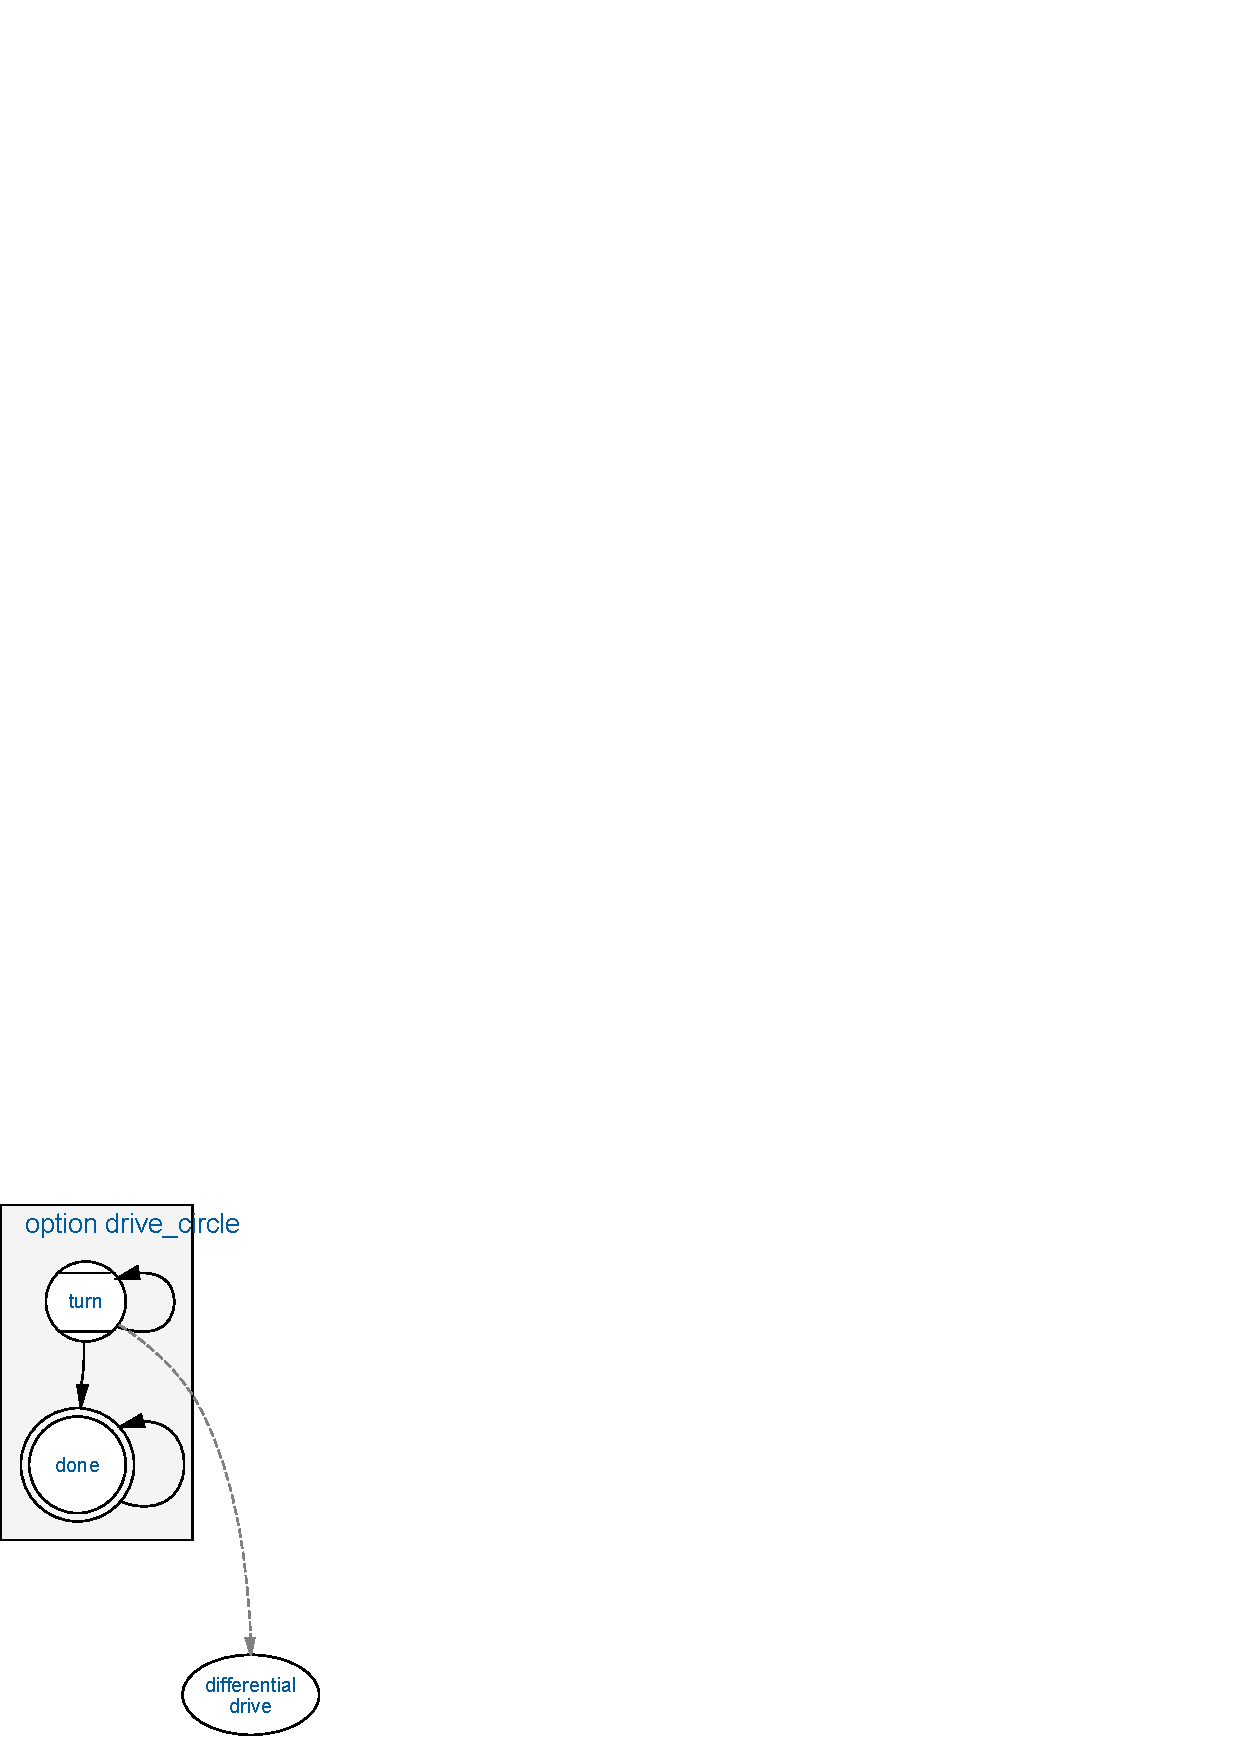
\includegraphics[width=.6\columnwidth]{../files/option_drive_circle.png}
    \label{fig:simpleFsm}
    \caption{An example of a figure generated by the XABSL compiler, from XABSL code.}
\end{figure}

\subsection{Difference with other specification possibilities}
There are many alternatives to XABSL, when it comes to defining a robot's
behavior. This section will discuss some of the alternatives, that had to be
considered before choosing XABSL.

\subsubsection{POSH}
POSH \cite{brom2006posh} is a very similar alternative implementation of a Behavior Specification
Language. Posh is defined as a \textit{Behavior Oriented Design}, which is
created from a combination of \textit{Object Oriented Design} (OOD, used by object oriented
programming languages like Java and C++) and \textit{Behavior Based Artificial
Intelligence} (BBAI). The BBAI-part of it is the decomposition of intelligence
as subtasks called \textit{acts}. Examples of acts are knowing your position and
planning a route. From OOD, BOD takes building your behavior in an object-hierarchy
and an agile and iterative development process.

POSH is an abbreviation of Parallel-rooted, Ordered, Slip-stack Hierarchical,
which, freely interpreted, stands for something that enables a user to specify
an agent's goals and priorities. This is actually quite similar to XABSL,
because it makes certain decisions, and then selects an action to be executed by
an external program. There are some important differences though:

\begin{itemize}
    \item POSH is designed to be used by non-pro\-gram\-mers. This means the
    interface is easy, colorful and simple, whereas XABSL prioritizes complex
    capabilities, making the specification somewhat more complex for
    non-programmers.
    \item Where XABSL has a close coupling with the perception stream of the
    robot, POSH has no variable management, enabling the system to be a lot
    easier to use, but also maximizing the complexity of the specified behaviors
    to a lower maximum than XABSL offers.
\end{itemize}

\subsubsection{The next thing}
I don't know yet, let's see tomorrow
%TODO

\subsection{XABSL specification}
XABSL makes use of four components: Agents, Options, states and Basic behavior.
The following subsections will explain what these are, and how they can be used.

\subsection{Agents}
An XABSL agent is a rooted acyclic graph, containing all the behaviors for one
agent. In this research, one agent will equal one robot. 



\begin{itemize}
\item \emph{Agents:} A rooted acyclic graph, containing all the behaviors for one
agent. Several of these agents can be created, all having their own graph and
thus their own behavior.
\item \emph{Options:} Complex agent behavior. Each option is on itself a finite
state machine, containing several states.
\item \emph{States:} `Actions' that can be either active or inactive. At least
one state is always active. Each option has an initial state, being the first
state to be active. States are connected with each other by decision trees,
deciding what state or option is activated next.
\item \emph{Basic behavior:} At every leaf of an option (so, every state with no
other states to reference to) a basic behavior is activated. This is a small
piece of C++ code, that influences actions of the agent. 
\end{itemize}



\subsubsection{Motivation to use it}
Using FSM's for behavior is an easily comprehensible method to specify behavior.
The advantages of XABSL are that tools are delivered to make a hierarchy
documentation for your website (or anything else). For example, the FSM in
figure \ref{fig:simpleFsm} is automatically generated from XABSL code.

Using this representation, tweaking the behavior should become an easier task
resulting in better results for autonomous exploration.

% TODO
This section will be expanded with the following: 

\section{RoboCup Rescue}
\subsection{Description}
The project used in cooperation with the application, is UsarCommander.
UsarCommander\footnote{Available at
\url{http://www.jointrescueforces.eu/wiki/tiki-index.php}}, originally developed by Bayu Slamet, and extended by Arnoud
Visser and many others. This program takes care of connecting to USARSim (the
simulator used in the Robocup) and
makes the user able to easily get sensor data from the robots in it. It is also
possible to control the robots with several types of behavior, like
corridor-following, obstacle-avoidance, or tele-operation. The last of which
enables the operator to manually control the robots by hand, using an
interactive human interface.

Over time, the system has been expanded with many subprojects, for example one
implementing a SLAM
(Simultaneous Localisation And Mapping) algorithm, to make an accurate map from
the sensor data of several robots\cite{slamet2006manifoldslam}. All the information used and produced by
these subprojects can be accessed by other subprojects, resulting in an ideal
environment for creating new robot-controlling applications.

\subsection{Motivation to use it}
The main reason to use this program, instead of any other, to interface my
software with USARSim is that it has so many features. The presence of many
subprojects in the code, makes it possible to make a very efficient autonomous
exploration algorithm interfacing with the subprojects at hand. Without using UsarCommander all
the needed software should be taken from somewhere else, or implemented solely
for this purpose.

Other software for this purpose is available too. %TODO: Specify other programs

but since this is a bachelor
thesis on the University of Amsterdam, and this is the software used by it in
the RoboCup, this is the logical choice.
\section{Approach}
\begin{comment}
This section will contain my approach
\end{comment}

\subsection{Interfacing both programs}
Since the UsarCommander is written in Visual Basic, and the basic behaviors of
XABSL are written in C++, a bridge should be made. This is done by creating a
Dynamic Link Library (DLL). This DLL contains the needed functions of the C++
program, making them accessible for Visual Basic. The bridge works both ways, so
Visual Basic can offer output symbols to the XABSL Engine, while the engine can
offer input symbols to the agent.

\subsection{Creating a succesful hierarchy}
This section will tell about the FSM hierarchy I will make for autonomous
exploration


\section{Results}
This section will contain results, hopefully in the form of explored maps, numbers of victims found, etc.

\section{Conclusion}

%\end{multicols}{2}
\bibliography{bib}{}
\bibliographystyle{plain}
\end{document}

